\documentclass{article}

\usepackage{a4wide}
\usepackage[utf8]{inputenc}
\usepackage[T1]{fontenc}
\usepackage[french]{babel}
\usepackage[babel=true]{csquotes} % guillemets français
\usepackage{graphicx}
\graphicspath{{Images/}}
\usepackage{color}
\usepackage{hyperref}
\hypersetup{colorlinks,linkcolor=,urlcolor=blue}

\usepackage{amsmath}
\usepackage{amssymb}


\title{Devoir Programmation Concurrente}
\author{Matthias Coutin 36000206, L3 informatique}
\date{\today}

\begin{document}

\maketitle % pour écrire le titre


%% Le résumé:
\begin{abstract}
 Dans ce rapport j'expliquerai les étapes de la mise en oeuvre de l'exercice. L'exercice consistant à implémenter un objet File de façon à ce qu'elle puisse être gérée par des Threads,  en prenant en compte l'exclusion mutuelle, puis de créer un thread producteur et plusieurs Threads Consommateurs, le tout afficher dans une interface graphique.
\end{abstract}

\section{Conception de l'exercice}
\label{section:hello} % pour faire référence à la section ailleurs (\ref{...} voir plus bas)

Définition des objets clés de l'exercice.

Outils utilisés :
\begin{itemize}
\item \textit{Swing}~\cite{swingDoc}
  pour l'interface Java
\item \textit{Tkinter}~\cite{tkinterDoc} Pour l'interface Python
\end{itemize}
% \cite{...} permet de faire référence à des éléments de la
% bibliographie.

\subsection{Conception de la File}


Une File est un type de donnée où le stockage et l'accès est effectué 
par la règle FIFO ( First In First Out ), qui signifie le premier élément entrant et sera le premier sortant de la file. Pour son implémentation nous avons besoins : 
\begin{itemize}
\item De la taille de la file, le nombre d'éélément qu'elle contient
\item D'une fonction enfilé qui ajoute un élément en fin de file
\item Et d'une fonction défilé qui retire l'élément en début file
\item D'une fonction pour savoir si la file est vide
\item D'une fonction pour savoir si la file est pleine
\end{itemize}

La fonction file vide et nécessaire pour la fonction défilée car si la file est vide on ne peut pas retirer d'éléments, de même pour la fonction file pleine et enfilée, on ne peut pas ajouter un élément quand la file est pleine.


\subsection{Conception des Threads}


Les Threads qui seront créés sont un thread producteur et un thread consommateur qui se partageront la file comme ressource commune. Le thread Consommateur appellera la fonction défilée et le thread Producteur appellera la fonction empilée, mais pour pouvoir assurer l'exclusion mutuelle, l'utilisation d'un verrou est requis. Le principe était que quand le thread Consommateur accède à la ressource, la ressource est verrouillée pour le thread Producteur et inversement. De plus nous utiliserons les fonctions wait et notifyall pour mettre en attente le travail du thread Consommateur quand la file est vide et mettre en attente le travail du thread Producteur quand la file est pleine, la mise en attente d'un thread Consommateur sera suivie du réveil du thread Producteur et inversement. J'implémenterais aussi l'interruption des Threads. pour leurs arrêts.
 \subsection{Interface Graphique}
 L'affichage des différents éléments se fera comme suit :
 
 \begin{itemize}
\item Un label ( texte ) pour l'affichage de la file
\item Un label pour afficher le travail du Producteur
\item Un label pour afficher le travail du Consommateur
\item Un bouton d'arret et de reprise des Threads
\item Un bouton pour quitter le programme
\end{itemize}
 
\section{Implementation en Python et en Java}



\subsection{La Class File}
En Python :
\begin{center}
  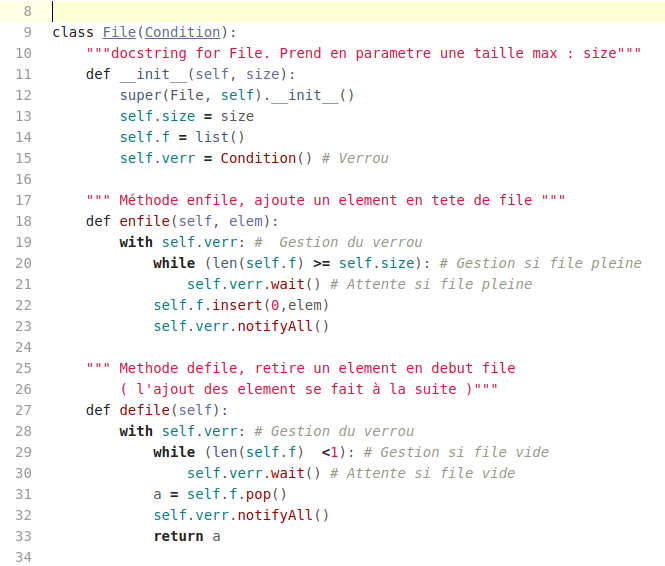
\includegraphics[scale=0.6]{FilePy.png}
\end{center}
En Java :
\begin{center}
  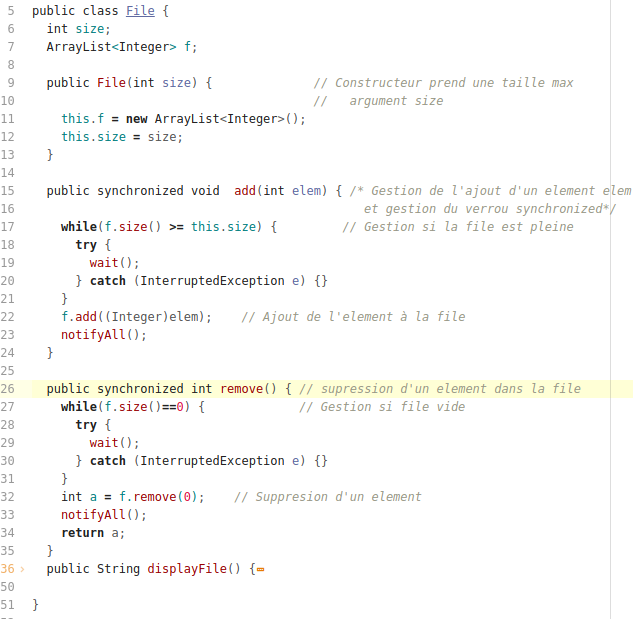
\includegraphics[scale=0.6]{Filejava.png}
\end{center}

\subsection{La Class Producteur et Consommateur}

En Python :
\begin{center}
  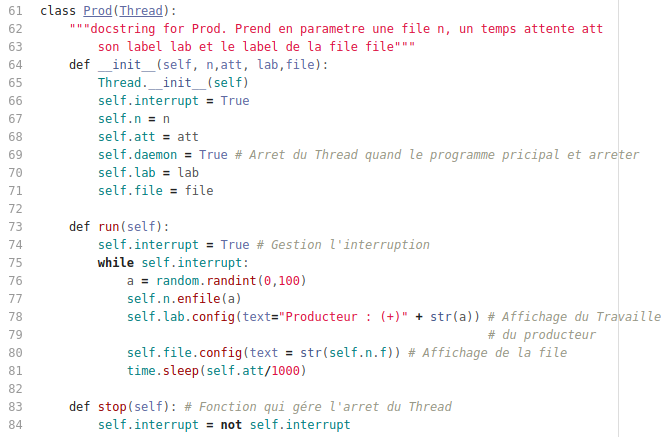
\includegraphics[scale=0.6]{Prodpy.png}
\end{center}
\begin{center}
  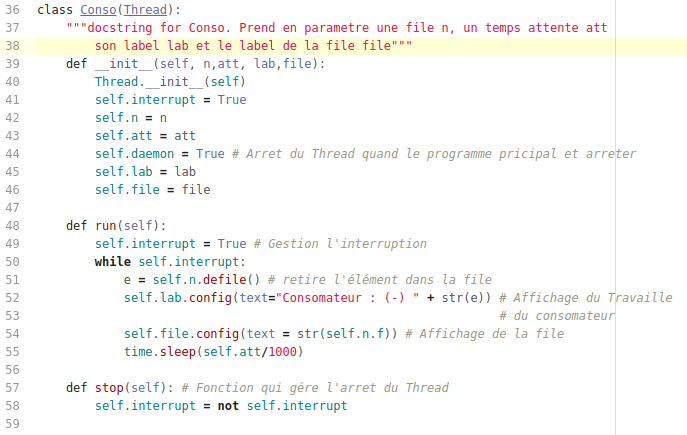
\includegraphics[scale=0.6]{Consopy.png}
\end{center}

En Java :
\begin{center}
  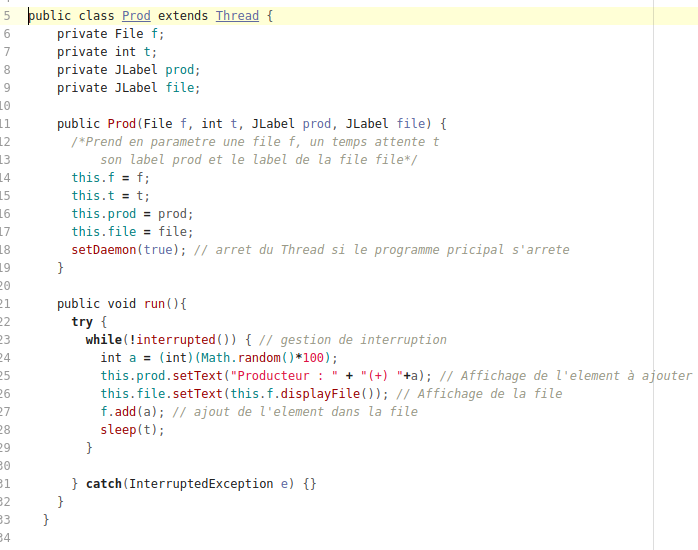
\includegraphics[scale=0.6]{Prodjava.png}
\end{center}
\begin{center}
  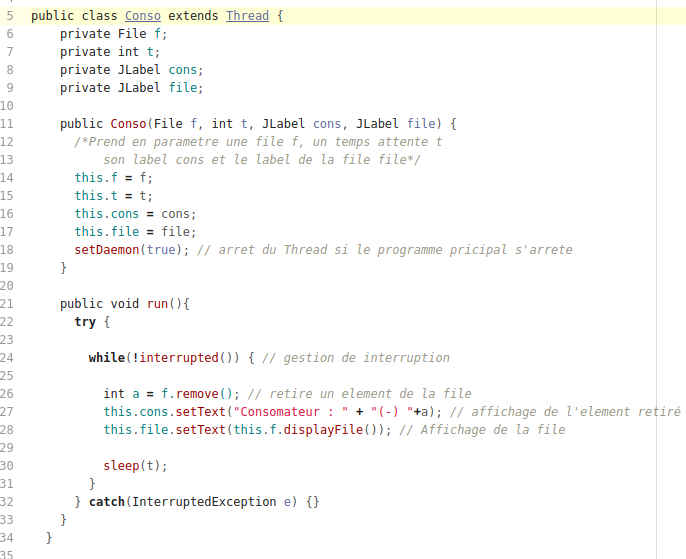
\includegraphics[scale=0.6]{Consojava.png}
\end{center}

\section{Résultat}

Affichage graphique des fênetres, des programmes en Python et Java :

En Python :
\begin{center}
  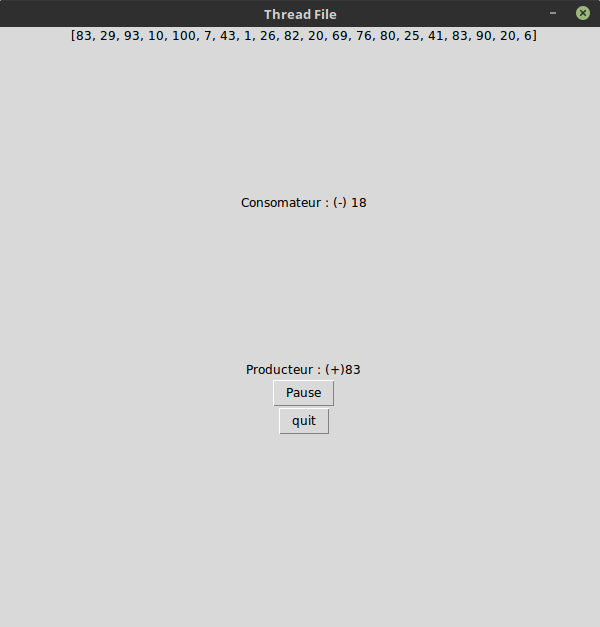
\includegraphics[scale=0.6]{Prgmpy.png}
\end{center}
En Java : 
\begin{center}
  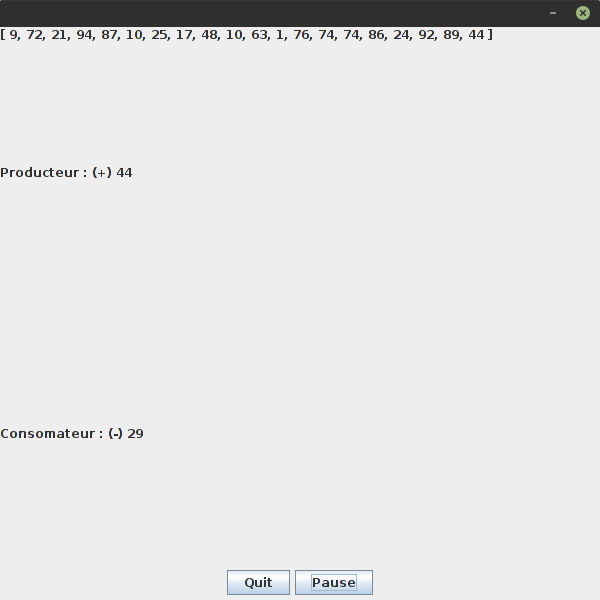
\includegraphics[scale=0.6]{Prgmjava.png}
\end{center}



%%% La bibliographie:
\bibliographystyle{plain}
\bibliography{ma_biblio}

\end{document}
